% LaTeX template for creating an MNRAS paper
%
% v3.2 released 20 July 2023
% (version numbers match those of mnras.cls)
%
% Copyright (C) Royal Astronomical Society 2015
% Authors:
% Keith T. Smith (Royal Astronomical Society)

%%%%%%%%%%%%%%%%%%%%%%%%%%%%%%%%%%%%%%%%%%%%%%%%%%%%%%%%%%%%%%%%%%%%%%%%%%%%%%%%%%%%%%%%%%%%%%%%%%%%
% Basic setup. Most papers should leave these options alone.
\documentclass[fleqn,usenatbib]{mnras}

% MNRAS is set in Times font. If you don't have this installed (most LaTeX
% installations will be fine) or prefer the old Computer Modern fonts, comment
% out the following line
\usepackage{newtxtext,newtxmath}
% Depending on your LaTeX fonts installation, you might get better results with one of these:
%\usepackage{mathptmx}
%\usepackage{txfonts}

% Use vector fonts, so it zooms properly in on-screen viewing software
% Don't change these lines unless you know what you are doing
\usepackage[T1]{fontenc}

% Allow "Thomas van Noord" and "Simon de Laguarde" and alike to be sorted by "N" and "L" etc. in the bibliography.
% Write the name in the bibliography as "\VAN{Noord}{Van}{van} Noord, Thomas"
\DeclareRobustCommand{\VAN}[3]{#2}
\let\VANthebibliography\thebibliography
\def\thebibliography{\DeclareRobustCommand{\VAN}[3]{##3}\VANthebibliography}


%%%%% AUTHORS - PLACE YOUR OWN PACKAGES HERE %%%%%

% Only include extra packages if you really need them. Avoid using amssymb if newtxmath is enabled, as these packages can cause conflicts. newtxmatch covers the same math symbols while producing a consistent Times New Roman font. Common packages are:
\usepackage{graphicx}	
\usepackage{amsmath}	
\usepackage{physics}
\usepackage{enumitem}
\usepackage{anyfontsize}
\usepackage{placeins}
\usepackage{cleveref}


%%%%%%%%%%%%%%%%%%%%%%%%%%%%%%%%%%%%%%%%%%%%%%%%%%%%%%%%%%%%%%%%%%%%%%%%%%%%%%%%%%%%%%%%%%%%%%%%%%%%

%%%%% AUTHORS - PLACE YOUR OWN COMMANDS HERE %%%%%

% Please keep new commands to a minimum, and use \newcommand not \def to avoid
% overwriting existing commands. Example:
%\newcommand{\pcm}{\,cm$^{-2}$}	% per cm-squared

\graphicspath{{images/}}
%\raggedbottom               %This will let the height of the textblock vary from page to page. 

% Command to use placeins with \subsection
\makeatletter
\AtBeginDocument{%
  \expandafter\renewcommand\expandafter\subsection\expandafter
    {\expandafter\@fb@secFB\subsection}%
  \newcommand\@fb@secFB{\FloatBarrier
    \gdef\@fb@afterHHook{\@fb@topbarrier \gdef\@fb@afterHHook{}}}%
  \g@addto@macro\@afterheading{\@fb@afterHHook}%
  \gdef\@fb@afterHHook{}%
}
\makeatother

%%%%%%%%%%%%%%%%%%%%%%%%%%%%%%%%%%%%%%%%%%%%%%%%%%%%%%%%%%%%%%%%%%%%%%%%%%%%%%%%%%%%%%%%%%%%%%%%%%%%


%%%%%%%%%%%%%%%%%%% TITLE PAGE %%%%%%%%%%%%%%%%%%%%%%%%%%%%%%%%%%%%%%%%%%%%%%%%%%%%%%%%%%%%%%%%%%%%%

% Title of the paper, and the short title which is used in the headers.
% Keep the title short and informative.
\title[]{Simulating the formation of super-massive binaries following galactic mergers}

% The list of authors, and the short list which is used in the headers.
% If you need two or more lines of authors, add an extra line using \newauthor
\author[Marco Bianchi]{
Marco Bianchi
\\
% List of institutions
University of Milano-Bicocca, Physics Department, Astrophysics and Space Physics master degree\\
Dynamics of Stellar Systems 2023-2024
}

% Enter the current year, for the copyright statements etc.
\pubyear{2025}

% Don't change these lines
\begin{document}
\label{firstpage}
\pagerange{\pageref{firstpage}--\pageref{lastpage}}
\maketitle

% Abstract of the paper
\begin{abstract}
  \large The Cocoon Nebula (IC 5146) is an HII region embedded within the Barnard 168 absorption nebula, making it a prime target for studying dust extinction. 
  We obtained photometric images of IC 5146 using H$\alpha$ and H$\beta$ filters and analyzed the Balmer decrement to create a two-dimensional map of the color excess E(B-V), which serves as a proxy for dust column density. 
  Our results indicate a median E(B-V) of $\approx 0.461 \pm 0.008$ across the nebula, with a standard deviation of $\approx 0.34$. 
  A comparison with previous spectroscopic studies reveals a discrepancy in E(B-V) estimates, which we attribute to methodological differences in spatial sampling.\\
  Furthermore, given the nebula's nearly spherical morphology and its ionization by a single B0.5V-type star (BD+46 3474), we tested the Strömgren sphere model. 
  By incorporating literature values for electron density and temperature, as well as for the radius and temperature of BD+46 3474, we derived a Strömgren radius of $\approx 1.14$ pc, which is broadly consistent with the observed nebular size. 
  However, uncertainties in the nebula's distance and simplifying assumptions in the Strömgren model highlight the need for more detailed modeling.
\end{abstract} 
%%%%%%%%%%%%%%%%%%%%%%%%%%%%%%%%%%%%%%%%%%%%%%%%%%%%%%%%%%%%%%%%%%%%%%%%%%%%%%%%%%%%%%%%%%%%%%%%%%%%




%%%%%%%%%%%%%%%%% BODY OF PAPER %%%%%%%%%%%%%%%%%%%%%%%%%%%%%%%%%%%%%%%%%%%%%%%%%%%%%%%%%%%%%%%%%%%%

\section{Introduction}\label{sec:introduction}
A nebula is a region of the interstellar medium (ISM) that appears particularly bright (emission and reflection nebulae) or dark (absorption nebulae) with respect to its surroundings. 
Most emission nebulae originate from molecular clouds, the coldest and densest regions of the ISM, which tend to collapse under their own gravity, creating ideal conditions for star formation.
These stellar nurseries can host young stars hot enough to emit ultraviolet photons, which photoionize the surrounding hydrogen gas. 
Protons and electrons then recombine into excited atomic states. 
These atoms then transition to the ground state by emitting a cascade of photons, some of which escape the nebula and reach our telescopes.
The result of this process is a so-called HII region of fluorescent gas.
Since these nebulae are usually optically thick to Lyman-series photons ("case B" recombination), the most prominent emission lines arise from the H$\alpha$ ($n=3 \rightarrow$ 2) and H$\beta$ ($n=4 \rightarrow$ 2) Balmer transitions, which are located at $\lambda_{H\alpha} \approx 6563 \text{\r{A}}$ and $\lambda_{H\beta} \approx 4861 \text{\r{A}}$, respectively.
%%%%%%%%%%%%%%%%%%%%%%%%%%%%%%%%%%%%%%%%%%%%%%%%%%

\subsection{Dust extinction}\label{sec:dust_introduction}
The ISM is not only composed of gas but also contains solid particles, known as dust grains, which can absorb and scatter light.
In general, dust extinction $A(\lambda)$ at a given wavelength $\lambda$ can be expressed as the difference between the observed and emitted apparent magnitudes of the source:
\begin{equation}
  A(\lambda) = m(\lambda)_\text{obs} - m(\lambda)_\text{emit} \:\: \Rightarrow \:\: 
  f_\text{obs} (\lambda) = 10^{-0.4 A(\lambda)} f_\text{emit} (\lambda) \, ,
  \label{eq:dust_extinction}
\end{equation}
where $f(\lambda)$ indicates a flux.

Dust extinction becomes more severe toward the blue end of the visible spectrum, causing the observed light to appear redder. 
The exact wavelength dependence of extinction is given by an empirical dust attenuation law $k(\lambda)$, based on a set of assumptions about the properties of the dust grains and the geometry of the system, which is related to extinction by: 
\begin{equation}
  A(\lambda) = k(\lambda) \text{E(B-V)} \:\: \Rightarrow \:\: 
  f_\text{obs} (\lambda) = 10^{-0.4 k(\lambda) \text{E(B-V)}} f_\text{emit} (\lambda) \, ,
  \label{eq:dust_attenuation_law}
\end{equation}
where E(B-V) is a parameter, called color excess.

Dust extinction of emission nebulae can be estimated by studying the so-called "Balmer decrement", i.e., the ratio of the H$\alpha$ and H$\beta$ emission lines, which is expected to increase beyond the intrinsic value of $\approx 2.86$ \citep{Osterbrock_1989}. In particular, the color excess E(B-V) can be obtained from Eq. \ref{eq:dust_attenuation_law} as:
\begin{equation}
  \text{E(B-V)} \simeq \dfrac{2.5}{k(H\beta) - k(H\alpha)} \log_{10} \left\{ \dfrac{\left[{f(H\alpha) / f(H\beta)}\right]_\text{obs}}{2.86} \right\} \, ,
  \label{eq:balmer_decrement}
\end{equation}
where the coefficient in front is $\approx 1.97$ for both the dust attenuation law by \cite{Calzetti_2000} and that by \cite{Cardelli_1989} with the parameter $R_V = 5$. 
The former law was originally derived for star-forming galaxies and is the most used in literature, while the latter was derived for the Milky Way, with $R_V = 3.1$ for diffuse ISM (the coefficient becomes $\approx 2.33$) and $R_V = 5$ for dense clouds.
Determining the optimal dust attenuation law for HII regions is still an active area of research, see \cite{Lin_2024} for a brief overview.
For more information on dust extinction theory, see chapter 12 of \cite{Boselli_2011}.

\begin{figure}\centering
	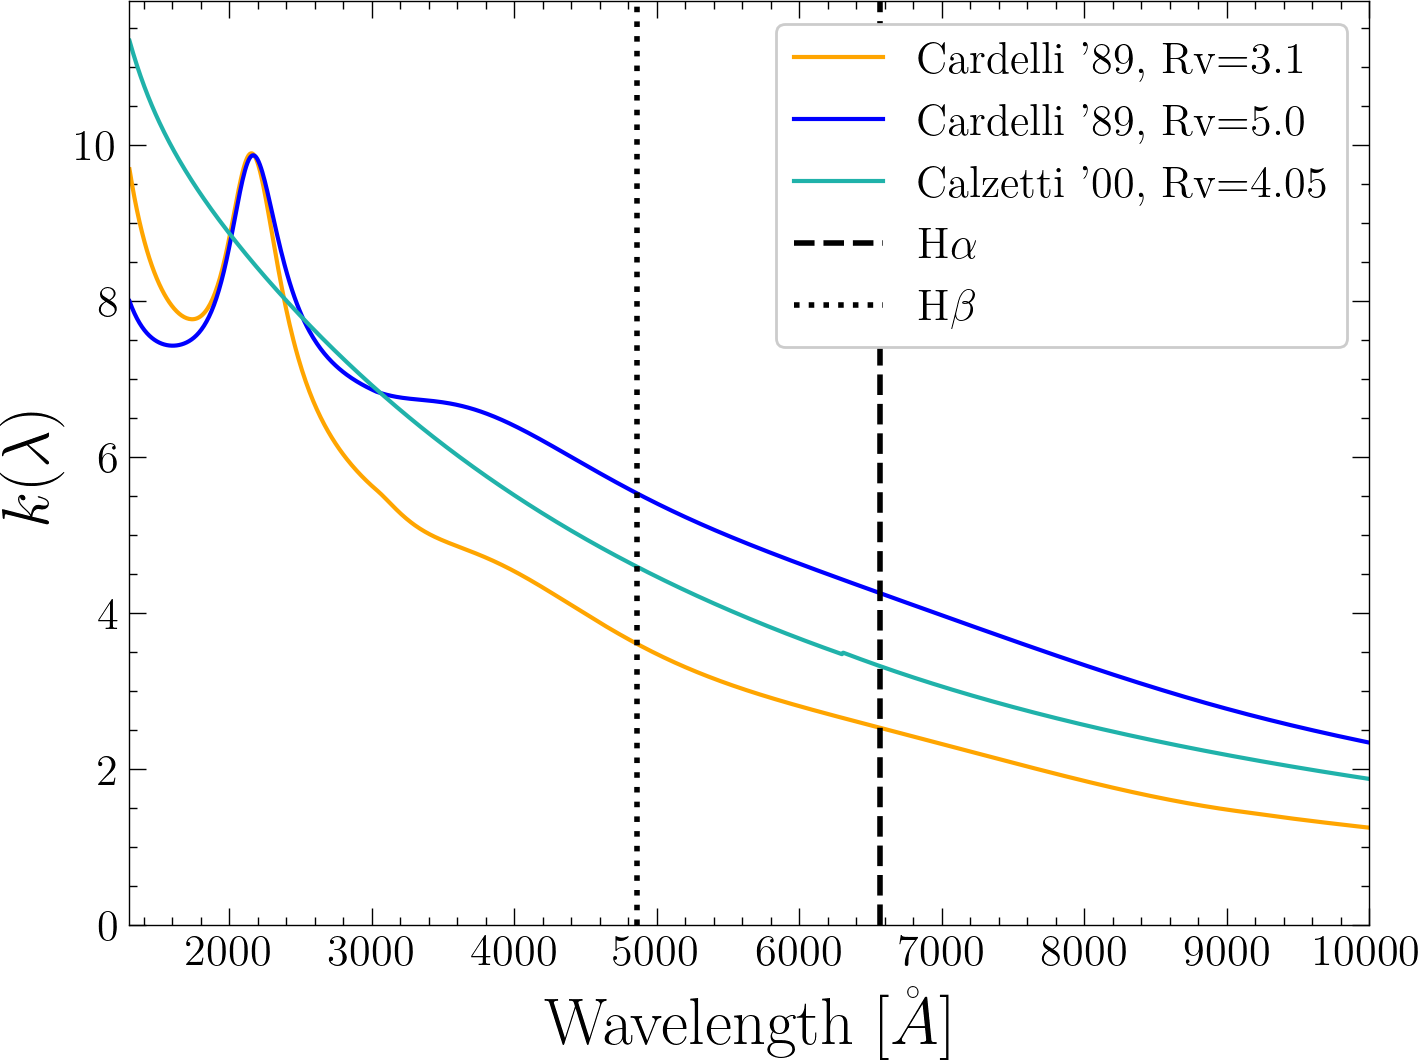
\includegraphics[width=0.85\columnwidth]{dust_attenuation_laws.png}
    \caption{Dust attenuation laws mentioned in the text.}
    \label{fig:dust_attenuation_laws}
\end{figure}
%%%%%%%%%%%%%%%%%%%%%%%%%%%%%%%%%%%%%%%%%%%%%%%%%%

\subsection{Strömgren sphere}\label{sec:stromgren_introduction}
HII regions are often spherically symmetric, with the ionizing star located at the center of the nebula.
\cite{Stromgren_1939} developed a simple model to describe the structure of these regions, assuming that the hydrogen gas is uniform and fully ionized within a certain radius $r_S$, known as Strömgren radius, and neutral outside of it, with a sharp transition between the two regions.
The Strömgren radius can be estimated by balancing the rate of ionization of hydrogen atoms by the star with the rate of recombination of protons and electrons.
The number of ionizing photons emitted by the star per unit time is given by:
\begin{equation}
  Q \left(H^0\right) = \int^\infty_{\frac{13.6\,\text{eV}}{h}} \dfrac{L_\nu}{h\nu} d\nu \, = \,
  4\pi R^2 \int^\infty_{\frac{13.6\,\text{eV}}{h}} \dfrac{f_\nu}{h\nu} d\nu \, ,
  \label{eq:photons_per_unit_time}
\end{equation}
where $f_\nu$ is the flux per unit frequency of the star.
We assume that the gas is optically thick to ionizing photons, meaning that all of them are absorbed.
The recombination rate per unit volume of neutral hydrogen plasma is $n_e n_{H^+} \alpha_B \simeq n_e^2 \alpha_B$, where $\alpha_B$ is the recombination coefficient for the so-called "case B" (recombinations to the ground state are not considered, because each emitted Lyman photon excites another atom) and is given by:
\begin{equation}
  \alpha_B \simeq 2.54 \times 10^{-13} \left(T/10^4 \text{K}\right)^{-0.8163} \text{cm}^3 \text{s}^{-1} \, .
  \label{eq:recombination_coefficient}
\end{equation}
The Strömgren radius can be estimated as:
\begin{equation}
  Q \left(H^0\right) = \dfrac{4\pi}{3} r_S^3 n_e^2 \alpha_B \left(T\right) 
  \:\: \Rightarrow \:\:
  r_S = \left( \dfrac{3 Q \left(H^0\right)}{4\pi n_e^2 \alpha_B \left(T\right)} \right)^{1/3} \, .
  \label{eq:stromgren_radius}
\end{equation}
This simple model has been improved over the years to account for more realistic conditions, such as the presence of dust \citep{Petrosian_1972} and non-spherical geometries \citep{McCullough_2000}, but it remains a useful tool for studying HII regions.
%%%%%%%%%%%%%%%%%%%%%%%%%%%%%%%%%%%%%%%%%%%%%%%%%%

\subsection{The HII region IC 5146}\label{sec:ic5146_introduction}
This work focuses on the Cocoon Nebula (IC 5146), an HII region located at approximately $800$ pc from Earth, in the Cygnus constellation (RA: 21h 53m 29.3s, Dec:+47° 14’ 46”), with a diameter of roughly 4.5 pc. 
It is a region of active star formation, containing many young stellar objects, yet the central B0.5V-type star (BD+46 3474) is the only one capable of ionizing the surrounding gas, making this nebula an excellent candidate for testing the Strömgren model.
Lastly, IC 5146 is embedded within the absorption nebula Barnard 168, a dense cloud of gas and dust that obscures background stars, making the Cocoon nebula an ideal target for studying dust extinction.

\citet{Garcia-Rojas_2014} performed a long-slit spatially resolved spectroscopic analysis of IC 5146, estimating many useful properties of the nebula, such as the electron density $n_e \approx 100$ cm$^{-3}$, the electron temperature $T_e \approx 6500$ K, and the distance $d \approx 800 \pm 80$ pc.
They even estimated the average H$\beta$ reddening factor, defined as $c(H\beta) = 0.4 k(H\beta) \text{E(B-V)} \approx 0.88 \pm 0.06$, which corresponds to a color excess $<$E(B-V)$>$ $\approx 0.361 \pm 0.024$ using the dust attenuation law by \cite{Cardelli_1989} with $R_V = 5$.
They also collected the high-resolution optical spectrum of the central star, which, combined with a state-of-the-art stellar atmosphere code, allowed them to estimate the effective temperature $T_\text{star} \approx 30500 \pm 1000$ K and the radius $R_\text{star} \approx 5.2 \pm 0.2 \, R_\odot$.
%%%%%%%%%%%%%%%%%%%%%%%%%%%%%%%%%%%%%%%%%%%%%%%%%%
%%%%%%%%%%%%%%%%%%%%%%%%%%%%%%%%%%%%%%%%%%%%%%%%%%%%%%%%%%%%%%%%%%%%%%%%%%%%%%%%%%%%%%%%%%%%%%%%%%%%



\section{Observations and data reduction}\label{sec:observation}
The photometric observations were carried out using an Atik $16200$ CCD attached to the $0.4m$ Telescopio Ottico Bicocca (TOBi), located in Milan. 
The exposure times were $1 \times 900s + 4 \times 300s$ with the H$\alpha$ filter and $4 \times 1200s$ with the H$\beta$ filter. The images were taken under clear sky conditions, particularly the $900s$ in H$\alpha$, although light pollution in Milan is never negligible.
\smallskip

The data reduction followed a standard procedure, which we outline below for clarity:
\begin{itemize}[left=6pt]
  \item First, we corrected the images for bias, dark current, and flat-field effects using the median frame for each:
  \begin{equation}
    \text{Science} = \left[ \text{Image} - \left(\text{Dark} - \text{Bias}\right) \dfrac{\Delta t_\text{image}}{\Delta t_\text{dark}} - \text{Bias} \right] / \text{Flat} \, .
    \label{eq:data_reduction}
  \end{equation}
  \item The pixel counts were converted to electron rates by multiplying by the TOBi gain factor of $0.6$ $e/$ADU and dividing by the exposure time.
  \item To estimate the background level, we masked the nebula and the stars in each image and applied the \texttt{Background2D} function from the \texttt{photutils} package \citep{Bradley_2024}.
  This function computes a low-resolution grid using robust statistics for each box and interpolates it with a bicubic spline model (\texttt{BgkZoomInterpolator}), yielding a smooth background surface that we then subtracted from the image.
  \item The images were corrected for dithering and misalignments due to being taken on different nights.
  \item We stacked the five H$\alpha$ images to obtain a final median image and repeated the process for the four H$\beta$ images.
  \item Finally, we corrected for residual misalignments between the two filters.
\end{itemize}

After background subtraction, the histogram of pixel values resembles a Gaussian distribution centered at zero, with the sources superimposed on the right tail. 
Assuming that Poisson fluctuations of the background are the dominant source of uncertainty and the photon rate is high enough for the central limit theorem to apply, we estimated the pixel-wise uncertainty on the electron rate as the standard deviation of this Gaussian.
The fit was performed only on the left side of the peak, where the background dominates.
\smallskip

The calibration constants $C_\text{Hx}$ used to convert the pixel values (and uncertainties) from electron rates to physical fluxes are defined as:
\begin{equation}
  f_\text{Hx}\left[\text{erg}/s/\text{cm}^2/\text{\r{A}}\right] = 10^{-C_\text{Hx}} \times f_\text{Hx}\left[e/s\right] \, .
  \label{eq:calibration}
\end{equation}
To estimate these constants, we used the \texttt{astrometry.net} software \citep{Astrometry_2010} to determine the positions of 99 stars in the frame, both in pixels and celestial coordinates.
We then measured the electron rate of each star using the \texttt{aperture}\_\texttt{photometry} function from the \texttt{photutils} package \citep{Bradley_2024}, employing a circular aperture with a diameter three times the FWHM.
To obtain the physical flux of each star, we convolved its spectrum $f_{\text{star}, \lambda}$, provided by the \cite{Gaia_2023} catalog, with the CCD+filter transmission curve $T_\text{Hx}(\lambda)$, effectively computing a weighted average of the flux within the filter band:
\begin{equation}
  f_\text{Hx}\left[\text{erg}/s/\text{cm}^2/\text{\r{A}}\right] \simeq 
  \frac{\int T_\text{Hx}(\lambda) f_{\text{star}, \lambda}(\lambda) d\lambda}{\int T_\text{Hx}(\lambda) d\lambda} \, .
  \label{eq:flux_convolution}
\end{equation}
We selected the 99 stars to avoid both saturation (too bright) and low signal-to-noise ratio (too faint). 
Additionally, we excluded stars superimposed on the nebula and those in close proximity to other stars.
The calibration constants were determined by fitting the log-log data with a linear model, as shown in Fig.~\ref{fig:Calib_tot}. 

Assuming that line emission dominates over the continuum, we converted the fluxes per unit wavelength into the total emission-line fluxes by multiplying by the effective width of the filter band $\Delta \lambda_\text{Hx}$.
We adopted $\Delta \lambda_{\text{H}\alpha} = 35 \text{\r{A}}$ and $\Delta \lambda_{\text{H}\beta} = 55 \text{\r{A}}$, as provided by the manufacturer. 
Finally, we divided by the number of arcsec$^2$ per pixel, obtaining the surface brightness in units of erg/s/cm$^2$/arcsec$^2$.
The medians of the nebular surface brightness are $\approx 3.3 \times 10^{-15}$ and $\approx 0.7 \times 10^{-15}$ erg/s/cm$^2$/arcsec$^2$ for the H$\alpha$ and H$\beta$ filters, respectively, with pixel-wise uncertainties of $\approx 2.5 \times 10^{-15}$ and $\approx 1.6 \times 10^{-15}$ erg/s/cm$^2$/arcsec$^2$.

\begin{figure}\centering
	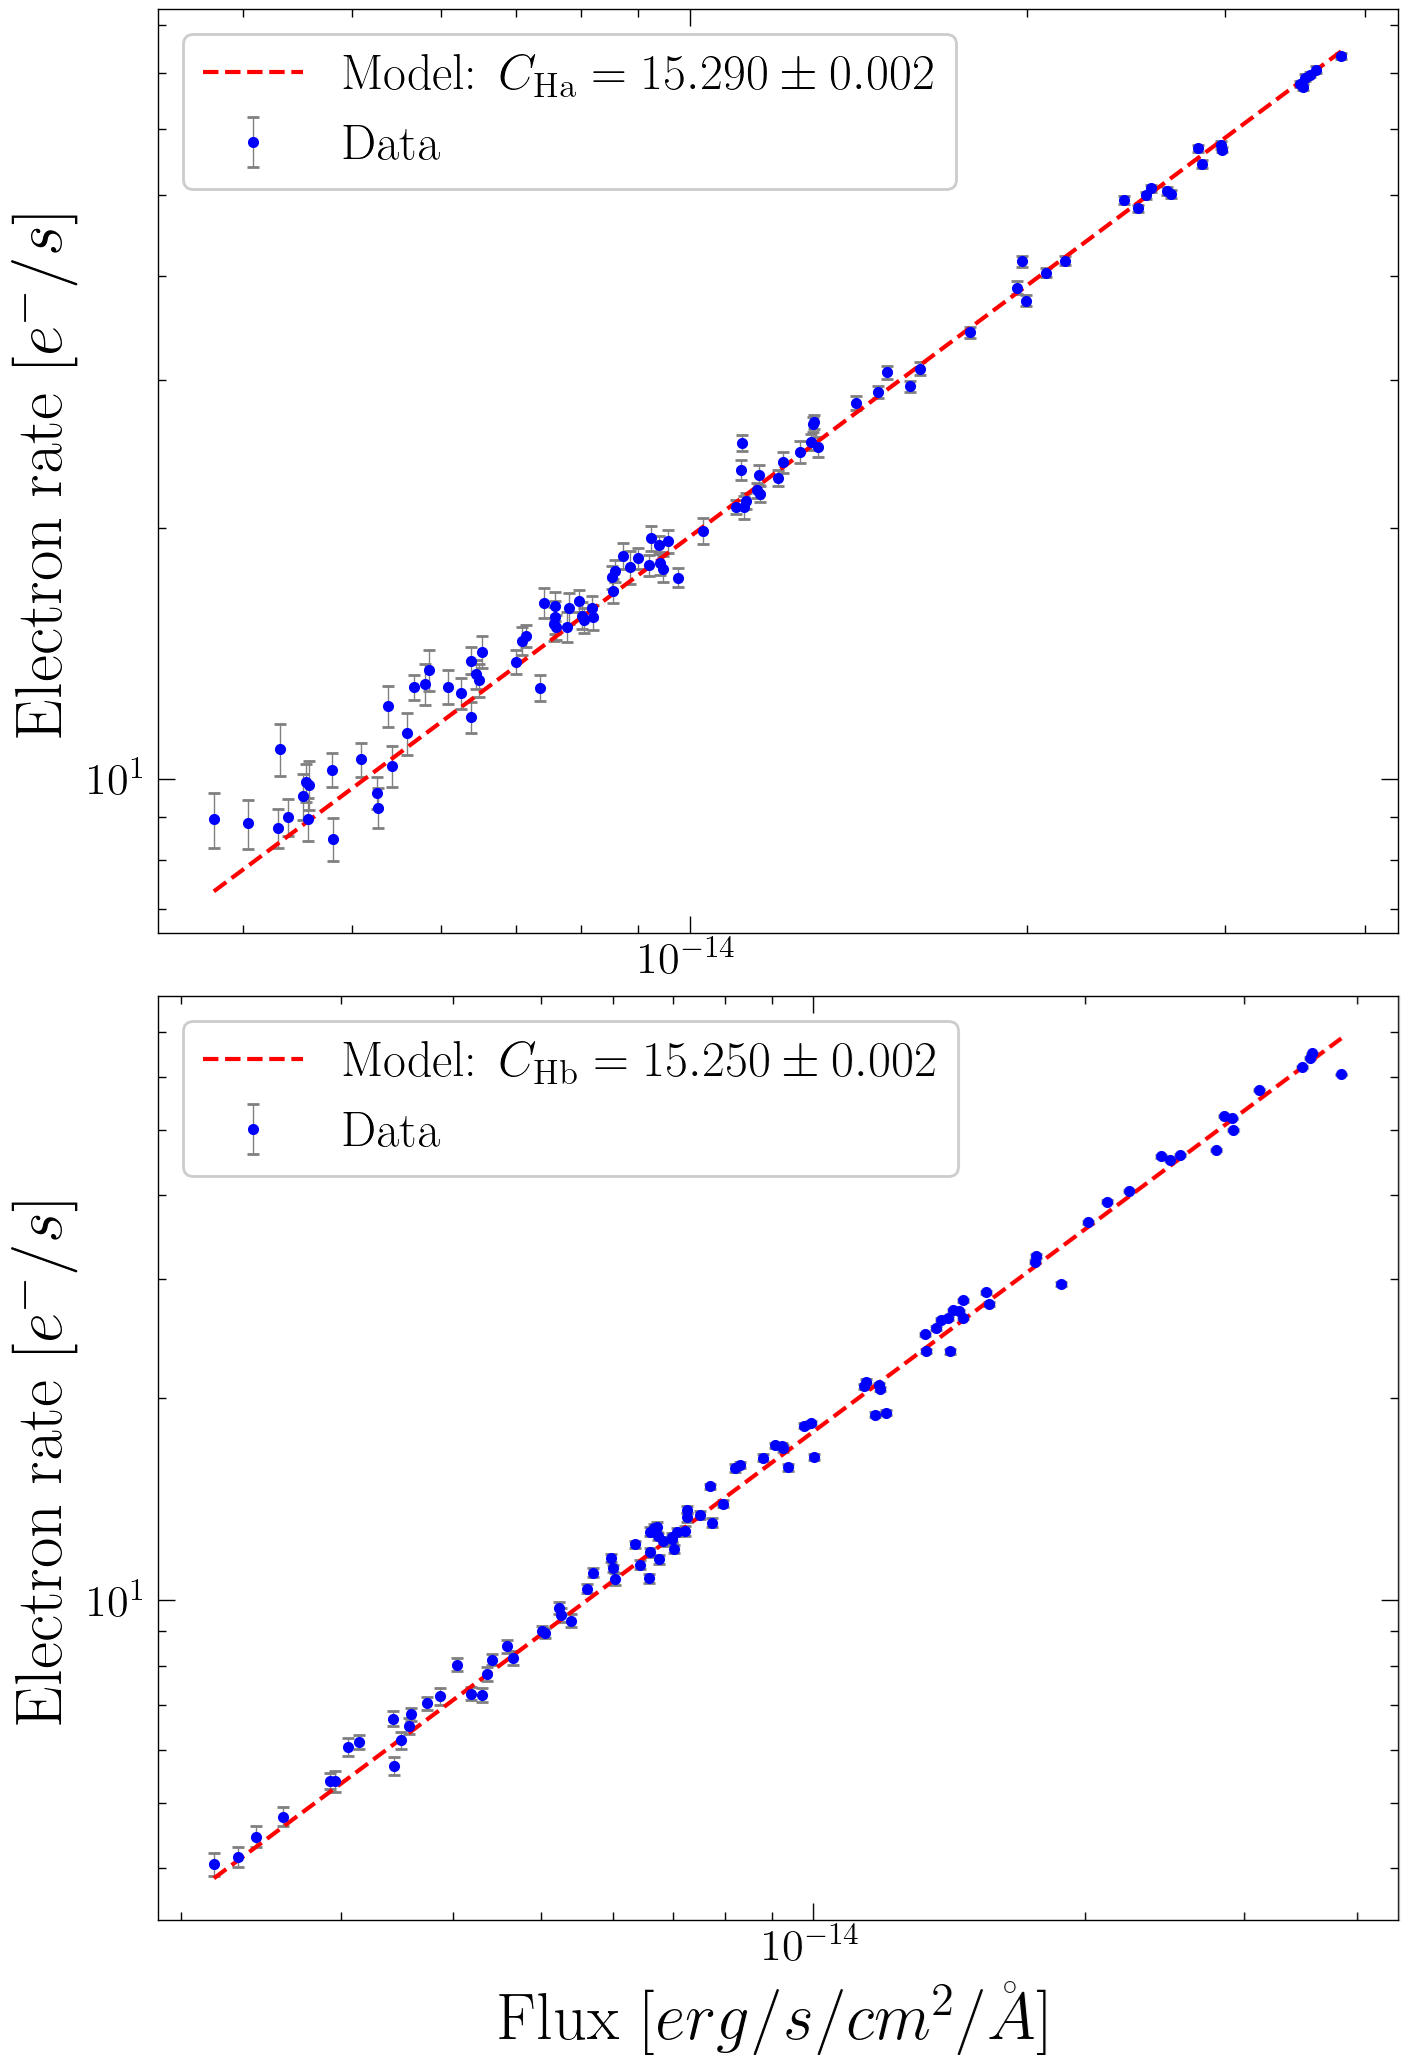
\includegraphics[width=0.7\columnwidth]{Calib_tot.png}
    \caption{Calibration constants for the H$\alpha$ (upper panel) and H$\beta$ (lower panel) filters to convert electron rates into physical fluxes, obtained by fitting the data from 99 stars with a linear model.}
    \label{fig:Calib_tot}
\end{figure}
%%%%%%%%%%%%%%%%%%%%%%%%%%%%%%%%%%%%%%%%%%%%%%%%%%
%%%%%%%%%%%%%%%%%%%%%%%%%%%%%%%%%%%%%%%%%%%%%%%%%%%%%%%%%%%%%%%%%%%%%%%%%%%%%%%%%%%%%%%%%%%%%%%%%%%%



\section{Results and discussion}\label{sec:results}
\subsection{Dust extinction map}\label{sec:dust_results}
We have seen in Sec.~\ref{sec:dust_introduction} that the color excess E(B-V) serves as a proxy for dust extinction.
Given a dust attenuation law, Eq. \ref{eq:balmer_decrement} allows us to estimate E(B-V) from the observed H$\alpha$ and H$\beta$ fluxes.
We approximated the coefficient in Eq. \ref{eq:balmer_decrement} as $\approx 1.97$, since this value closely matches those obtained using the dust attenuation laws of \cite{Calzetti_2000} and \cite{Cardelli_1989} with $R_V = 5$.
Initially, we attempted to estimate the pixel-wise E(B-V), but the uncertainties were too large to produce a meaningful map.
To mitigate this issue, we rebinned the pixels into $15 \times 15$ blocks and computed the median surface brightness for each block.
For the uncertainty, we adopted:
\begin{equation}
  \hat{\sigma}_\text{block} \simeq 1.253 \dfrac{\sqrt{\hat{\sigma}_\text{true values}^2 + \hat{\sigma}_\text{pixel}^2}}{\sqrt{N_\text{pixels in block}}} \, ,
  \label{eq:rebinning_uncertainty}
\end{equation}
where $\hat{\sigma}_\text{pixel}$ is the pixel-wise uncertainty estimated in Sec.~\ref{sec:observation}, $\hat{\sigma}_\text{true values}$ is the standard deviation of the pixel values within the block, and the coefficient $1.253$ accounts for the relationship between the uncertainty of the median and that of the mean in the limit of Gaussian distribution and large sample size. 
This rebinning allowed us to obtain a two-dimensional distribution of E(B-V) with satisfactory resolution and a signal-to-noise ratio (SNR) greater than $1$ for every block in the nebula, as shown in Fig~\ref{fig:EBV_image} and \ref{fig:SNR_EBV_image}.
\smallskip

The median E(B-V) across the entire nebula is $<\text{E(B-V)}> \approx 0.461 \pm 0.008$, with a standard deviation of $\approx 0.34$. 
This confirms the non-uniformity of the distribution shown in Fig.~\ref{fig:EBV_image}, further illustrated by the radial profile in Fig.~\ref{fig:EBV_profile}, where the median E(B-V) was computed over concentric annuli of equal area.
We compared our result with the independent spectroscopic estimate of $c(H\beta) = 0.4 k(H\beta) \text{E(B-V)} \approx 0.88 \pm 0.06$ from \cite{Garcia-Rojas_2014}.
Using the dust attenuation law of \cite{Cardelli_1989} with $R_V = 5$, they report $<\text{E(B-V)}> \approx 0.361 \pm 0.024$, which is inconsistent with our value.
In contrast, applying the \cite{Calzetti_2000} law yields $<\text{E(B-V)}> \approx 0.478 \pm 0.032$, which is in agreement.
However, these estimates are not directly comparable. 
Our value represents the median across the entire nebula, while theirs is an average over eight circular apertures positioned at increasing distances from the central star along a single direction. 
Given the clear asymmetry in the two-dimensional distribution of E(B-V), this methodological difference likely contributes to the observed discrepancy.
\smallskip

\begin{figure}\centering
	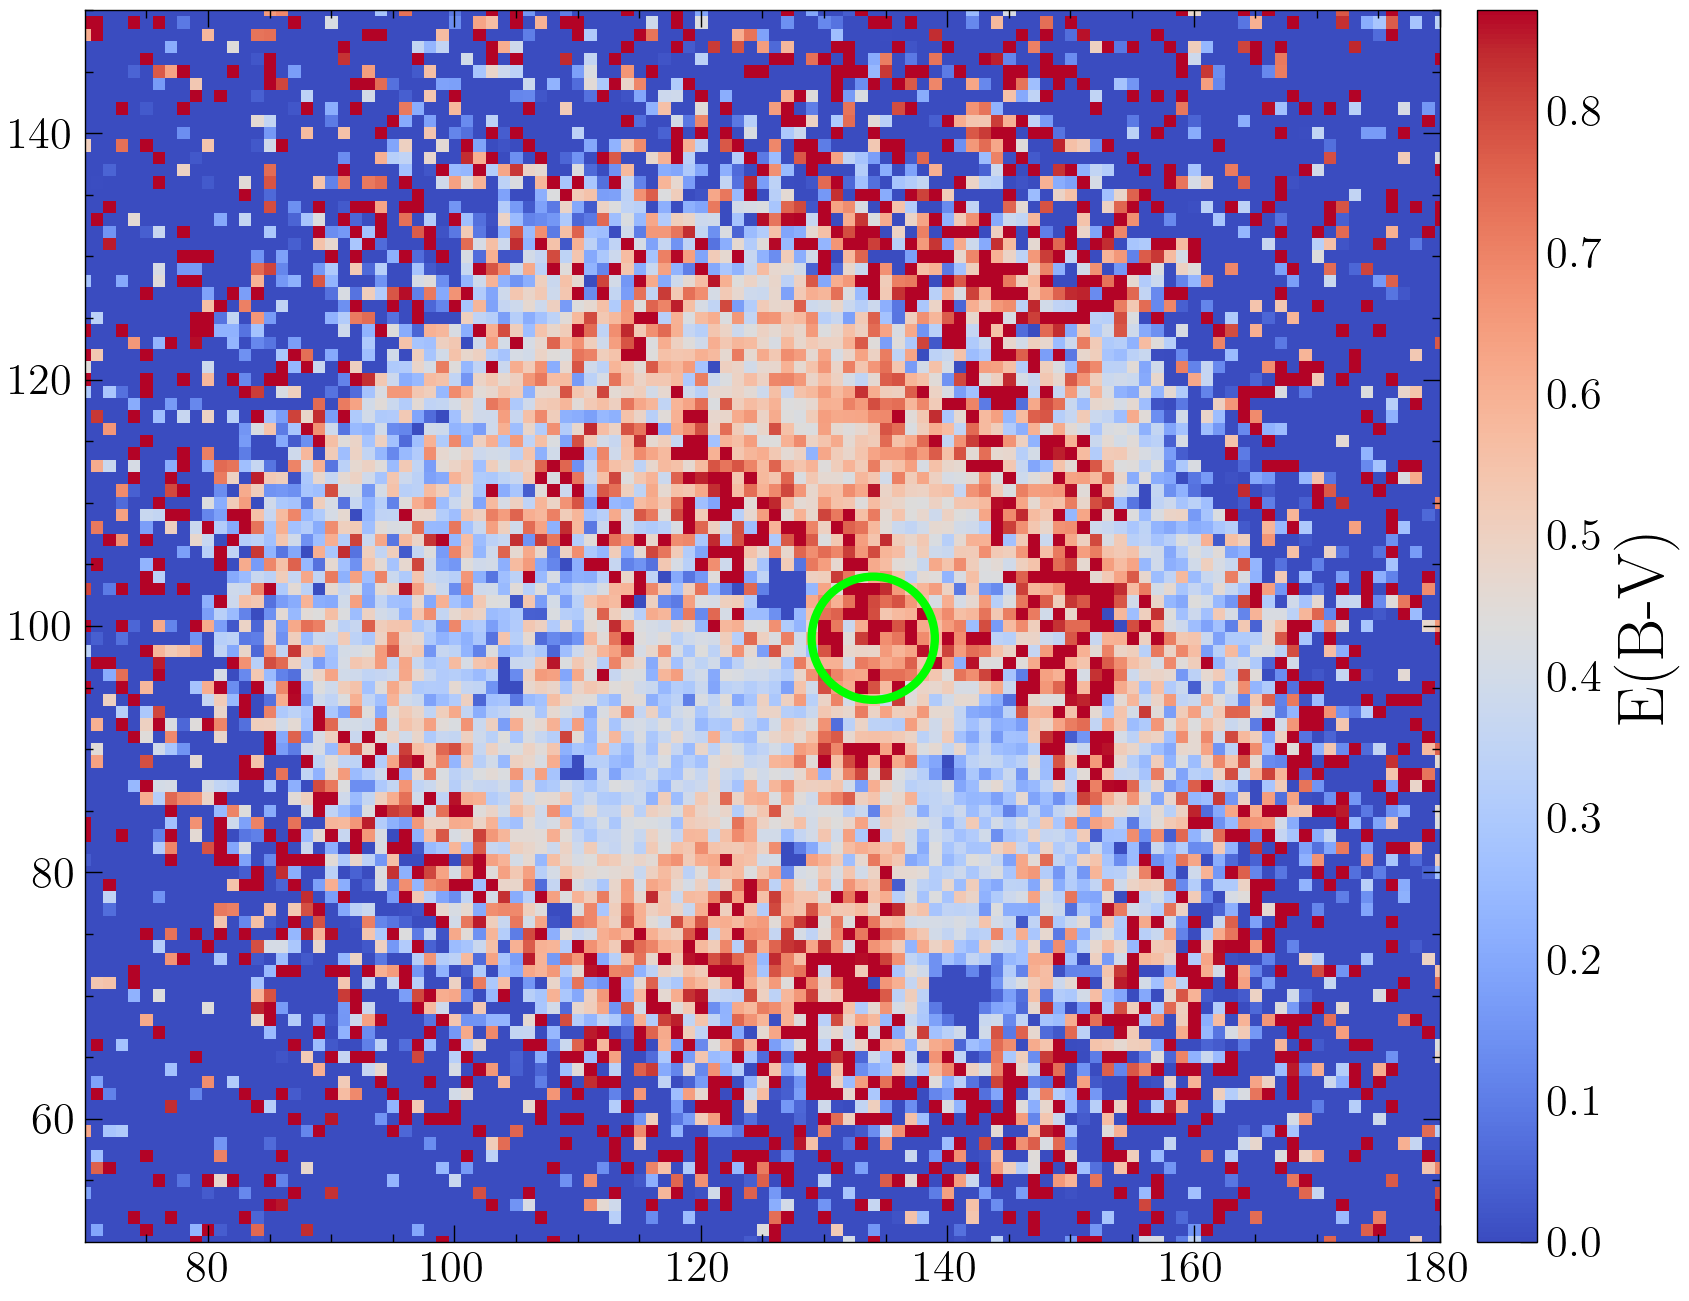
\includegraphics[width=0.94\columnwidth]{EBV_image.png}
    \caption{two-dimensional distribution of the color excess E(B-V) in IC 5146, based on rebinned pixels of size $15 \times 15$. 
    The green circle marks the region used to estimate the median E(B-V) near the central star.}
    \label{fig:EBV_image}
\end{figure}

\begin{figure}\centering
	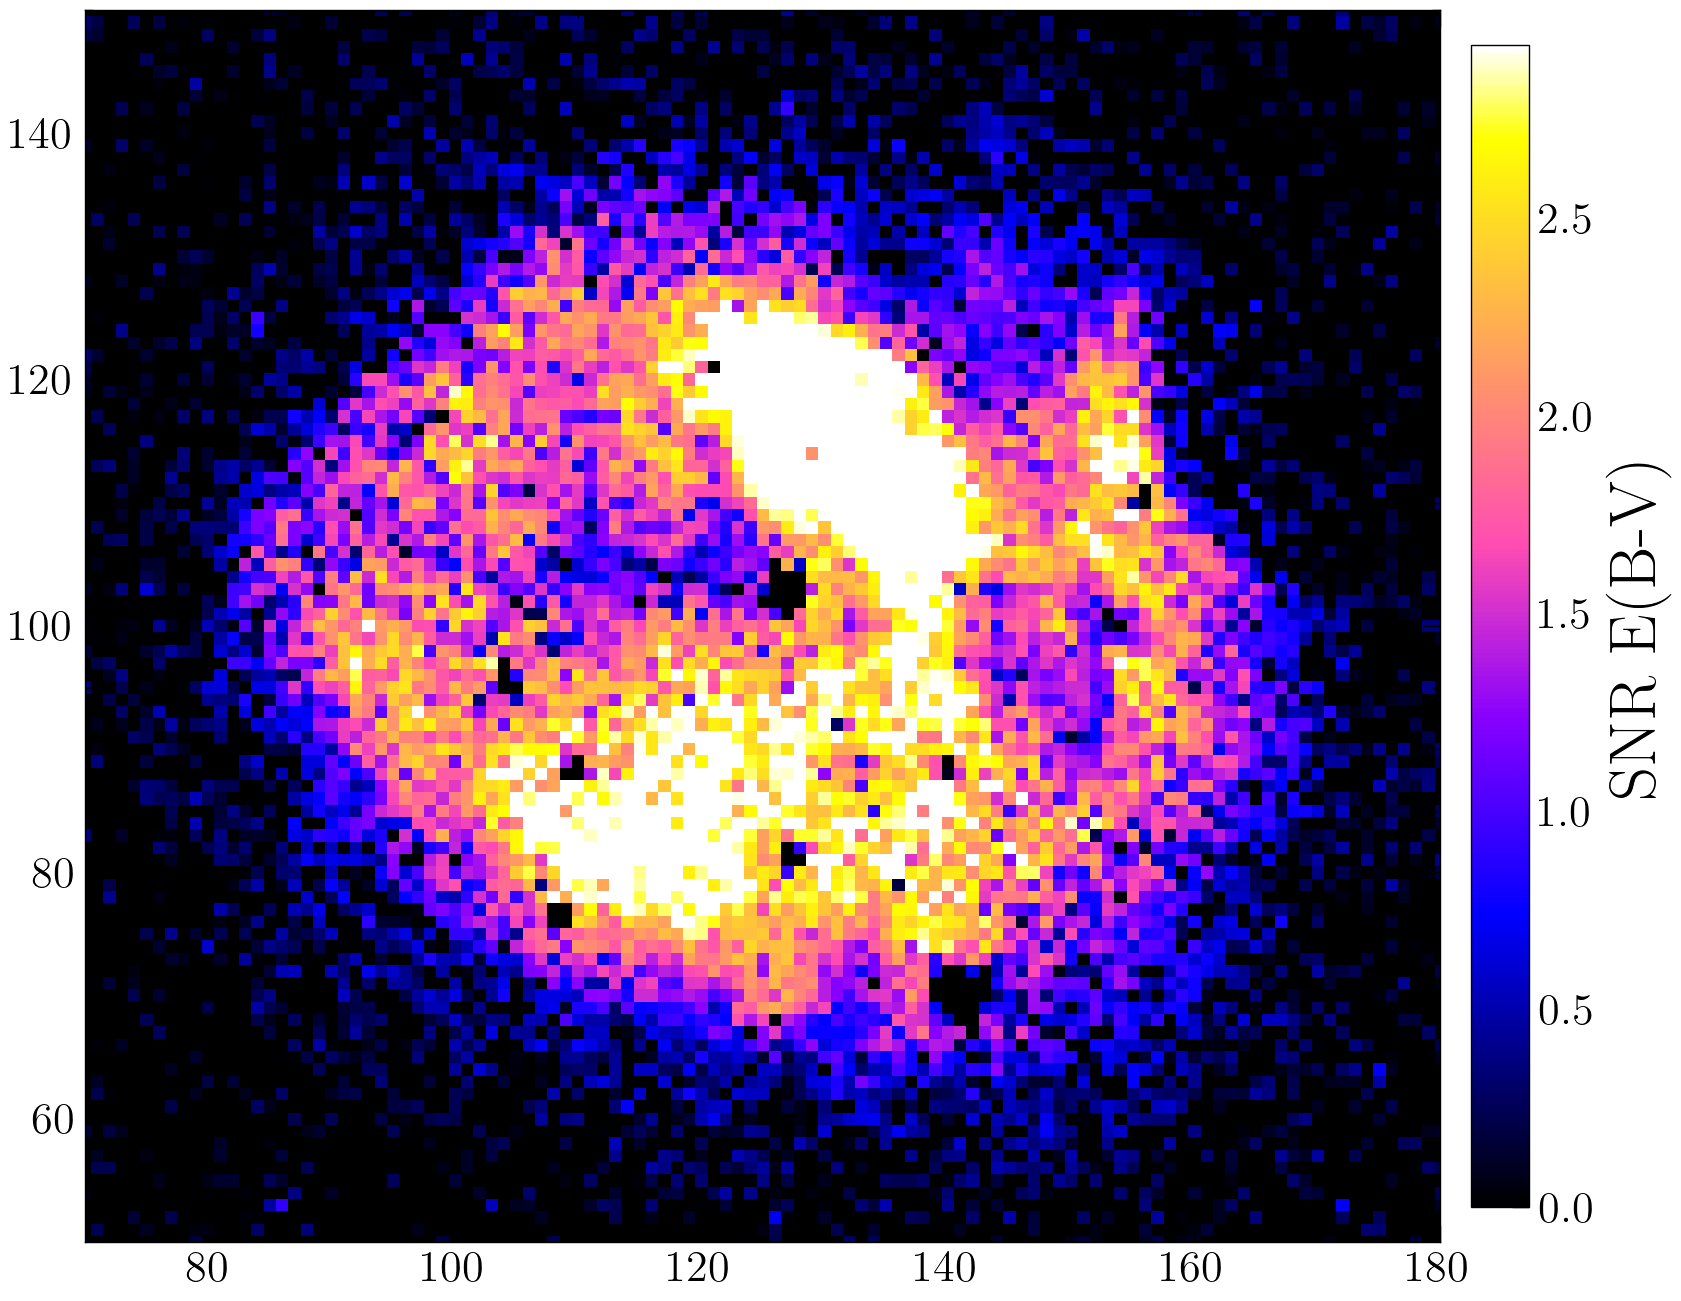
\includegraphics[width=0.94\columnwidth]{SNR_EBV_image.png}
    \caption{two-dimensional distribution of the signal-to-noise ratio of the color excess E(B-V) in IC 5146, based on rebinned pixels of size $15 \times 15$. }
    \label{fig:SNR_EBV_image}
\end{figure}

\begin{figure}\centering
	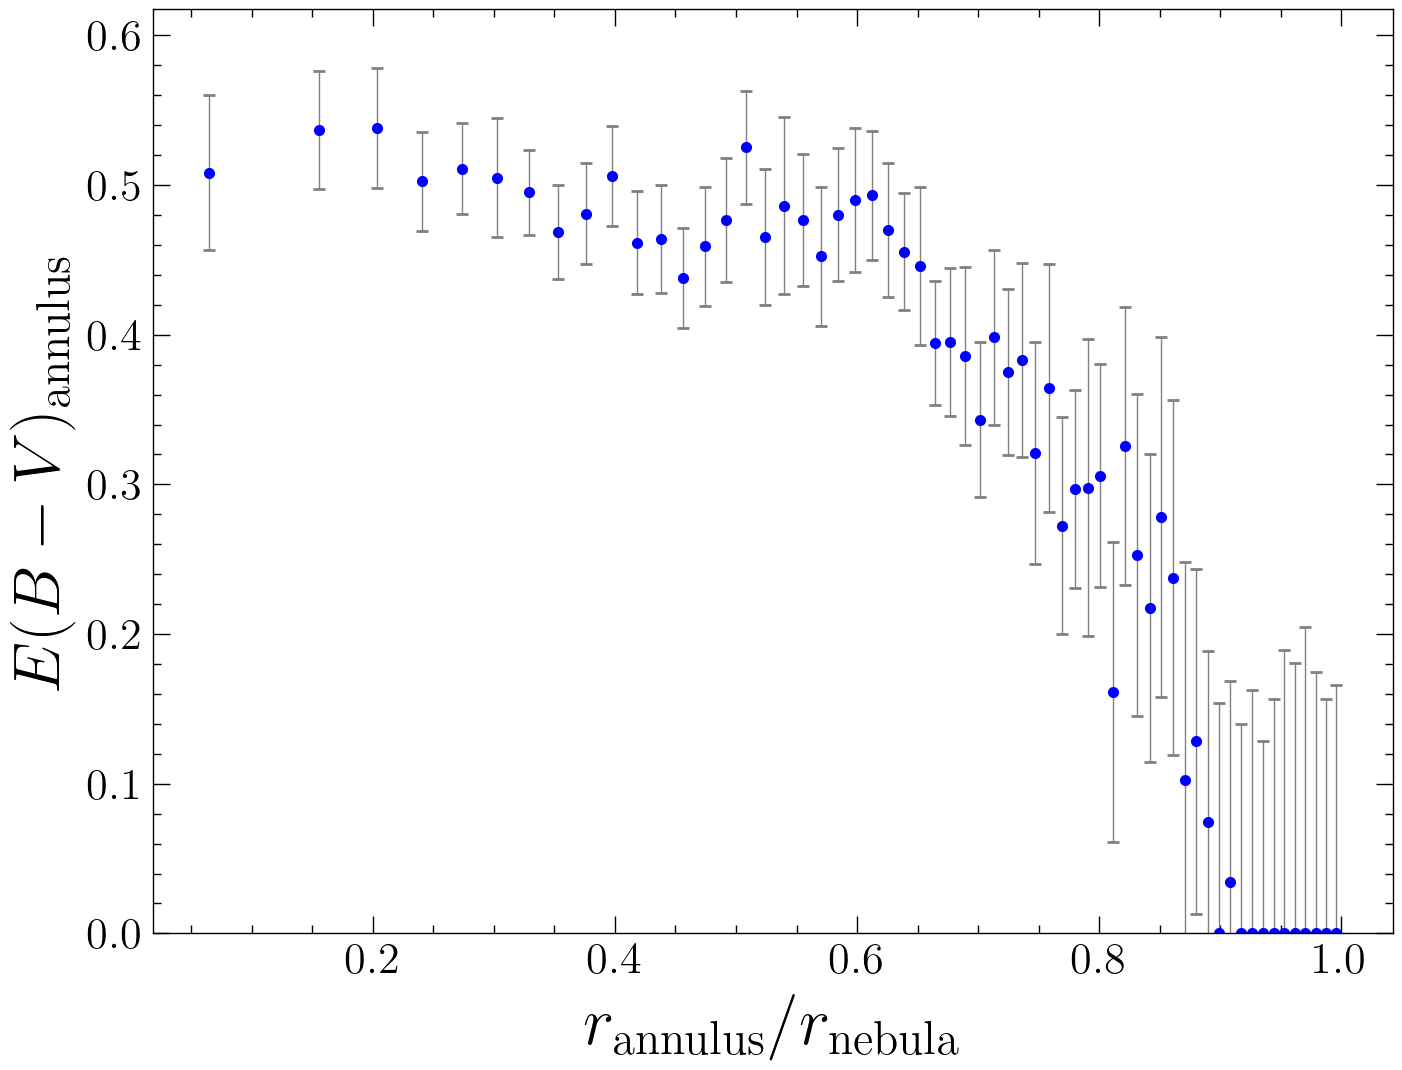
\includegraphics[width=0.7\columnwidth]{EBV_profile.png}
    \caption{Radial profile of the color excess E(B-V) in IC 5146. The points represent the median E(B-V) computed over concentric rings of equal area.}
    \label{fig:EBV_profile}
\end{figure}

As noted in Sec.~\ref{sec:ic5146_introduction}, we have reliable estimates for the temperature, radius, and distance of the central star.
Using these, we computed a blackbody spectrum that approximates the real spectrum of BD+46 3474 as:
\begin{equation}
  f_{BB, \lambda} (d) \simeq \pi \left(\frac{R_\text{star}}{d}\right)^2 B_\lambda (T_\text{star}) \, ,
  \label{eq:blackbody_spectrum}
\end{equation}
where $B_\lambda (T_\text{star})$ is the Planck function.
Since the estimates of $T_\text{star}$, $R_\text{star}$, and $d$ have associated uncertainties, we assumed their distributions to be Gaussian and performed Monte Carlo simulations to obtain the median and $90\%$ confidence interval of the blackbody spectrum.
We then compared this approximated spectrum with that observed by Gaia \citep{Gaia_2023}, after correcting for dust extinction using Eq. \ref{eq:dust_attenuation_law}.
To perform this correction, we computed the median E(B-V) over a circular aperture of radius $= 5$ blocks near the central star (as shown in Fig.~\ref{fig:EBV_image}), yielding $<\text{E(B-V)}>_{BD+46 3474} \approx 0.69 \pm 0.05$.
The result is highly sensitive to the choice of the dust attenuation law, and the one by \cite{Cardelli_1989} with $R_V = 5$ appears to be the only one compatible with the model, as shown in Fig.~\ref{fig:Spectrum_star}.
Notably, the estimate of $<\text{E(B-V)}>_{BD+46 3474}$ differs when using Cardelli's law with $R_V = 3.1$, since the coefficient in Eq. \ref{eq:balmer_decrement} is different.

\begin{figure}\centering
	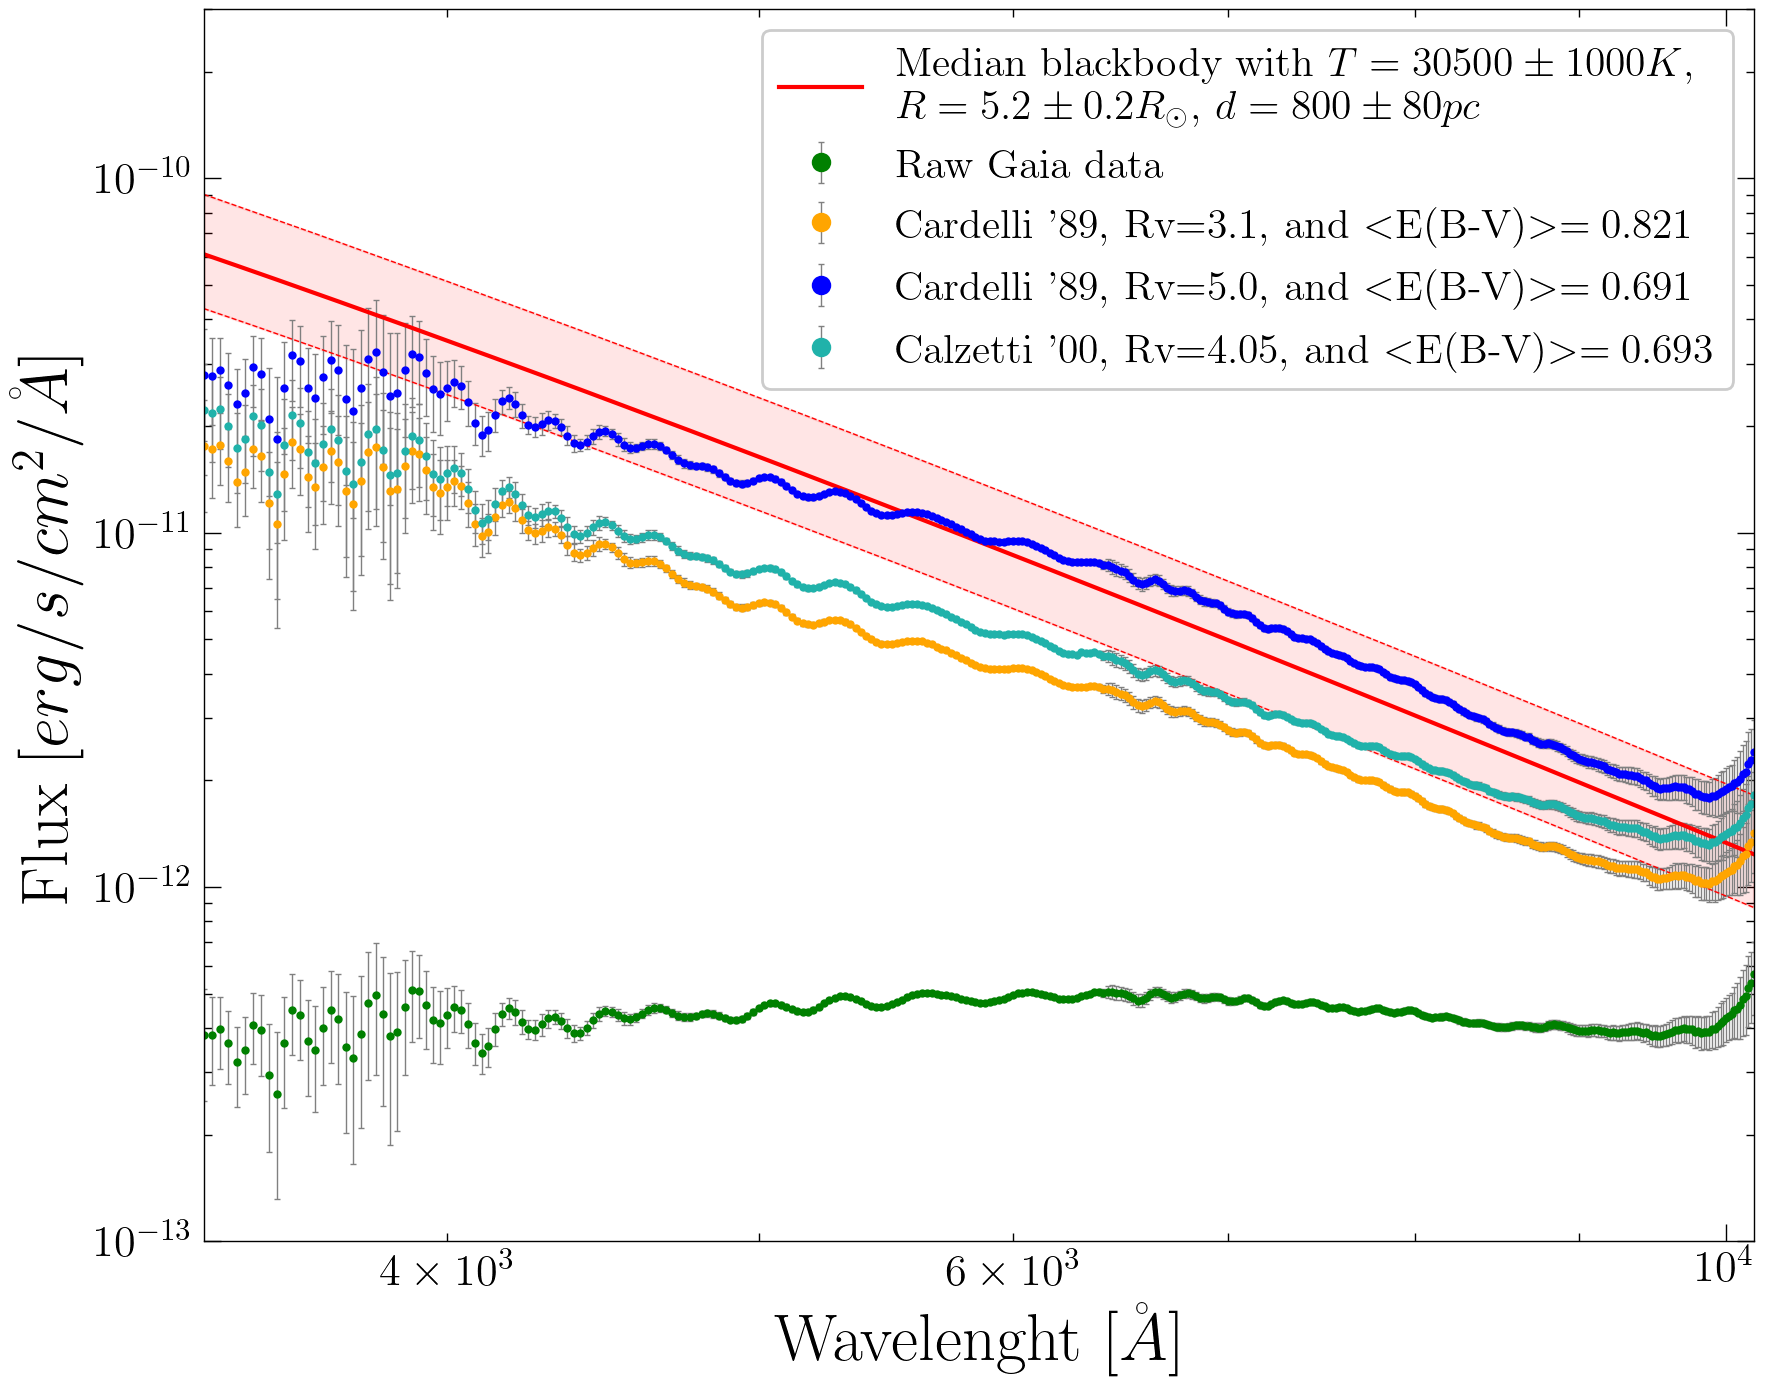
\includegraphics[width=0.9\columnwidth]{Spectrum_star_loglog.png}
    \caption{Comparison of the spectrum of the central star (BD +46 3474) as measured by Gaia (green), the same spectrum corrected for dust extinction using three different dust attenuation laws, and the blackbody spectrum computed using the star's temperature, radius, and distance as the star (red, with the 90$\%$ confidence interval).}
    \label{fig:Spectrum_star}
\end{figure}
%%%%%%%%%%%%%%%%%%%%%%%%%%%%%%%%%%%%%%%%%%%%%%%%%%

\subsection{Strömgren sphere}\label{sec:stromgren_results}
The Strömgren radius $r_S$ of IC 5146 can be estimated using Eq. \ref{eq:stromgren_radius}, provided that we know the electron density $n_e$, the electron temperature $T_e$, and the number of ionizing photons emitted by the central star per unit time $Q (H^0)$.
We already have spectroscopic estimates of the first two quantities from \cite{Garcia-Rojas_2014} (see Sec.~\ref{sec:ic5146_introduction}), while the third can be computed using Eq. \ref{eq:photons_per_unit_time}.
For this computation, we approximated the spectrum of BD+46 3474 as that of a spherical blackbody with radius $R_\text{star}$ and temperature $T_\text{star}$, obtaining $Q (H^0) \approx 6.6 \times 10^{47} \text{photons}/s$.
The resulting Strömgren radius is $r_S \approx 1.14$ pc, which is consistent with the size of the nebula, as shown in Fig.~\ref{fig:Stromgren}. 
To create this figure, we assumed that the nebula is located at a distance of $d \approx 800 \pm 80$ pc from Earth, as estimated by \cite{Garcia-Rojas_2014}.
However, the distance to IC 5146 has historically been a subject of debate, with some estimates exceeding $1$ kpc.
This uncertainty may partially explain why our estimate of the Strömgren radius is only half of what we expected, being roughly one-fourth of the typical literature value of $4.5$ pc for the diameter of the Cocoon nebula.

Finally, we emphasize that the Strömgren model is a simplification, as the actual structure of HII regions is more complex.
Factors such as the presence of dust, non-spherical geometries, and empty cavities created by the strong stellar winds of massive, hot stars like BD+46 3474 should be considered to give a complete description.


\begin{figure}\centering
	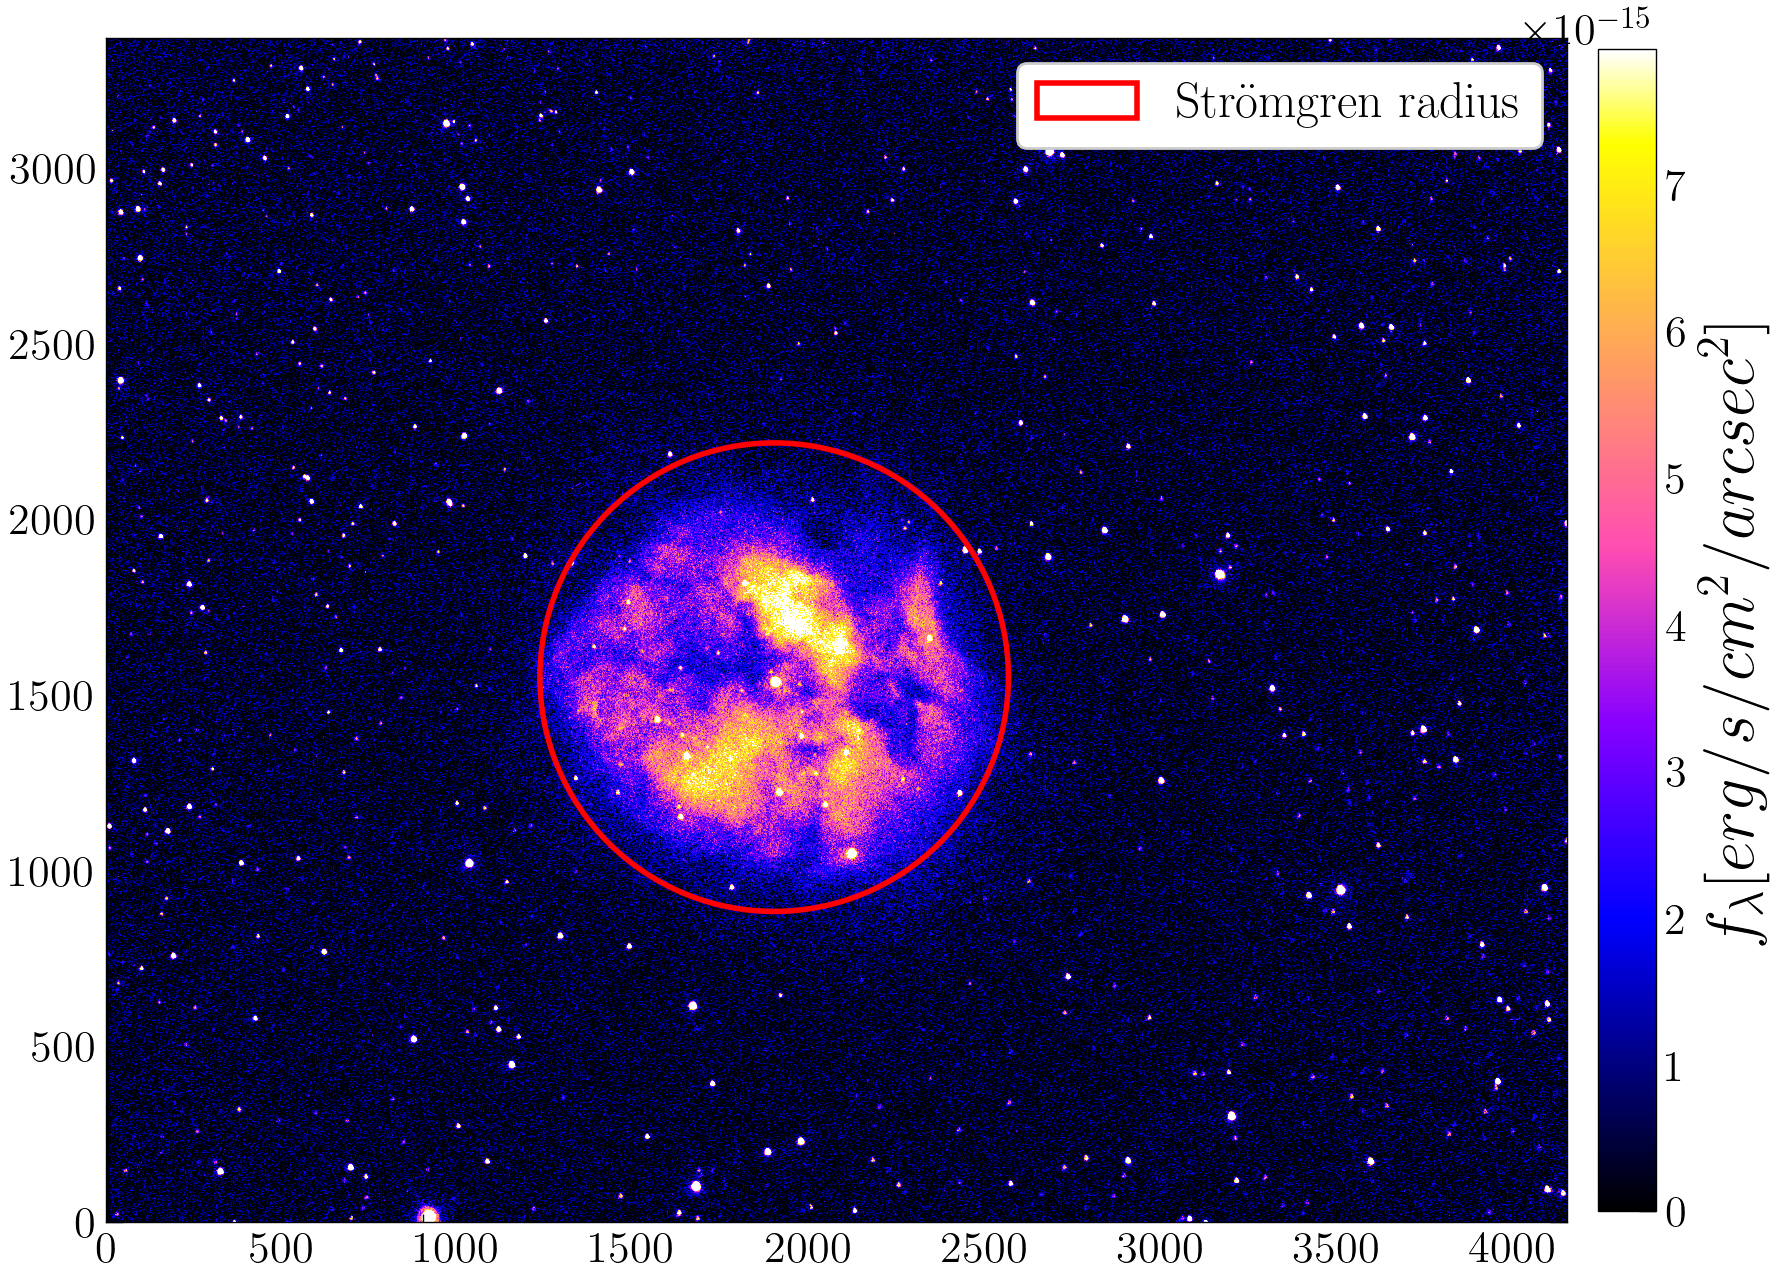
\includegraphics[width=0.98\columnwidth]{Stromgren.png}
    \caption{Image of IC 5146 in the H$\alpha$ filter. The red circle represents the Strömgren radius $r_S$.}
    \label{fig:Stromgren}
\end{figure}
%%%%%%%%%%%%%%%%%%%%%%%%%%%%%%%%%%%%%%%%%%%%%%%%%%
%%%%%%%%%%%%%%%%%%%%%%%%%%%%%%%%%%%%%%%%%%%%%%%%%%%%%%%%%%%%%%%%%%%%%%%%%%%%%%%%%%%%%%%%%%%%%%%%%%%%



\section{Conclusion}\label{sec:conclusion}
In this work, we analyzed the structure and dust extinction of the HII region IC 5146, using photometric observations in the H$\alpha$ and H$\beta$ narrow bands.

By constructing a two-dimensional map of the color excess E(B-V), which serves as a proxy for dust column density, we found a median value of $<\text{E(B-V)}> \approx 0.461 \pm 0.008$ across the nebula, with significant spatial variations.
To validate this estimate, we used it to correct the spectrum of the central star BD+46 3474, as measured by Gaia, and compared it to a blackbody spectrum computed from the star's temperature, radius, and distance.
This test showed that only the dust attenuation law by \cite{Cardelli_1989} with $R_V = 5$ is consistent with the model.
However, when comparing our result with the spectroscopic estimate from \cite{Garcia-Rojas_2014}, we found that the two values are only comparable when assuming \cite{Calzetti_2000}'s dust attenuation law, although the two estimates are not directly comparable due to methodological differences in spatial sampling.
These independent tests yield contradictory results regarding the choice of the dust attenuation law, emphasizing the need for further observations and modeling to fully understand the dust distribution in IC 5146.

We also tested the Strömgren model by estimating the Strömgren radius of IC 5146, finding $r_S \approx 1.14$ pc, which is consistent with the observed nebular size.
However, uncertainties in the nebula's distance and simplifying assumptions in the Strömgren model further highlight the need for more detailed modeling.

Unfortunately, we did not have time to collect our own spectroscopic data, using the TOBi spectrograph.
Such data would have allowed us to compute the ratios of collisionally excited forbidden lines, which depend on the electron density and temperature of the nebula.
This information would have been useful for independently determining these parameters, without relying on the literature.
%%%%%%%%%%%%%%%%%%%%%%%%%%%%%%%%%%%%%%%%%%%%%%%%%%
%%%%%%%%%%%%%%%%%%%%%%%%%%%%%%%%%%%%%%%%%%%%%%%%%%%%%%%%%%%%%%%%%%%%%%%%%%%%%%%%%%%%%%%%%%%%%%%%%%%%



\section{Appendix A: effective width of the H$\beta$ filter}\label{sec:appendix}
In this appendix, we address a potential systematic error in our analysis, arising from the effective width of the H$\beta$ filter.
The manufacturer provides values of $\Delta \lambda_{\text{H}\alpha} = 35 \text{\r{A}}$ and $\Delta \lambda_{\text{H}\beta} = 55 \text{\r{A}}$, which we used to convert fluxes per unit wavelength in the narrow filters into total emission-line fluxes, assuming that line emission dominates over the continuum.
However, the effective width of a photometric filter is typically, defined as:
\begin{equation}
  \Delta \lambda_\text{eff} = \dfrac{\int T(\lambda) d\lambda}{\max[{T(\lambda)}]} \, ,
  \label{eq:effective_width}
\end{equation}
where $T(\lambda)$ represents the transmission curve of the filter.
Using this definition, we obtain effective widths of $\Delta \lambda_{\text{H}\alpha} \approx 37.8 \text{\r{A}}$ (FMHW$_{\text{H}\alpha} \approx 36.6 \text{\r{A}}$) and $\Delta \lambda_{\text{H}\beta} \approx 104.8 \text{\r{A}}$ (FMHW$_{\text{H}\beta} \approx 98.0 \text{\r{A}}$).
While the estimate for the H$\alpha$ filter is consistent with the manufacturer's value, the one for the H$\beta$ filter is significantly larger.
This discrepancy could lead to an overestimation of the H$\beta$ flux, which would in turn critically affect the estimate of E(B-V), resulting in an almost complete absence of dust extinction in the nebula, contrary to expectations.
Additionally, we note that both narrow filters are not perfectly centered on the H$\alpha$ and H$\beta$ lines, as shown in Fig.~\ref{fig:Ha_transmission} and \ref{fig:Hb_transmission}, with the H$\beta$ filter being particularly shifted.

\begin{figure}\centering
	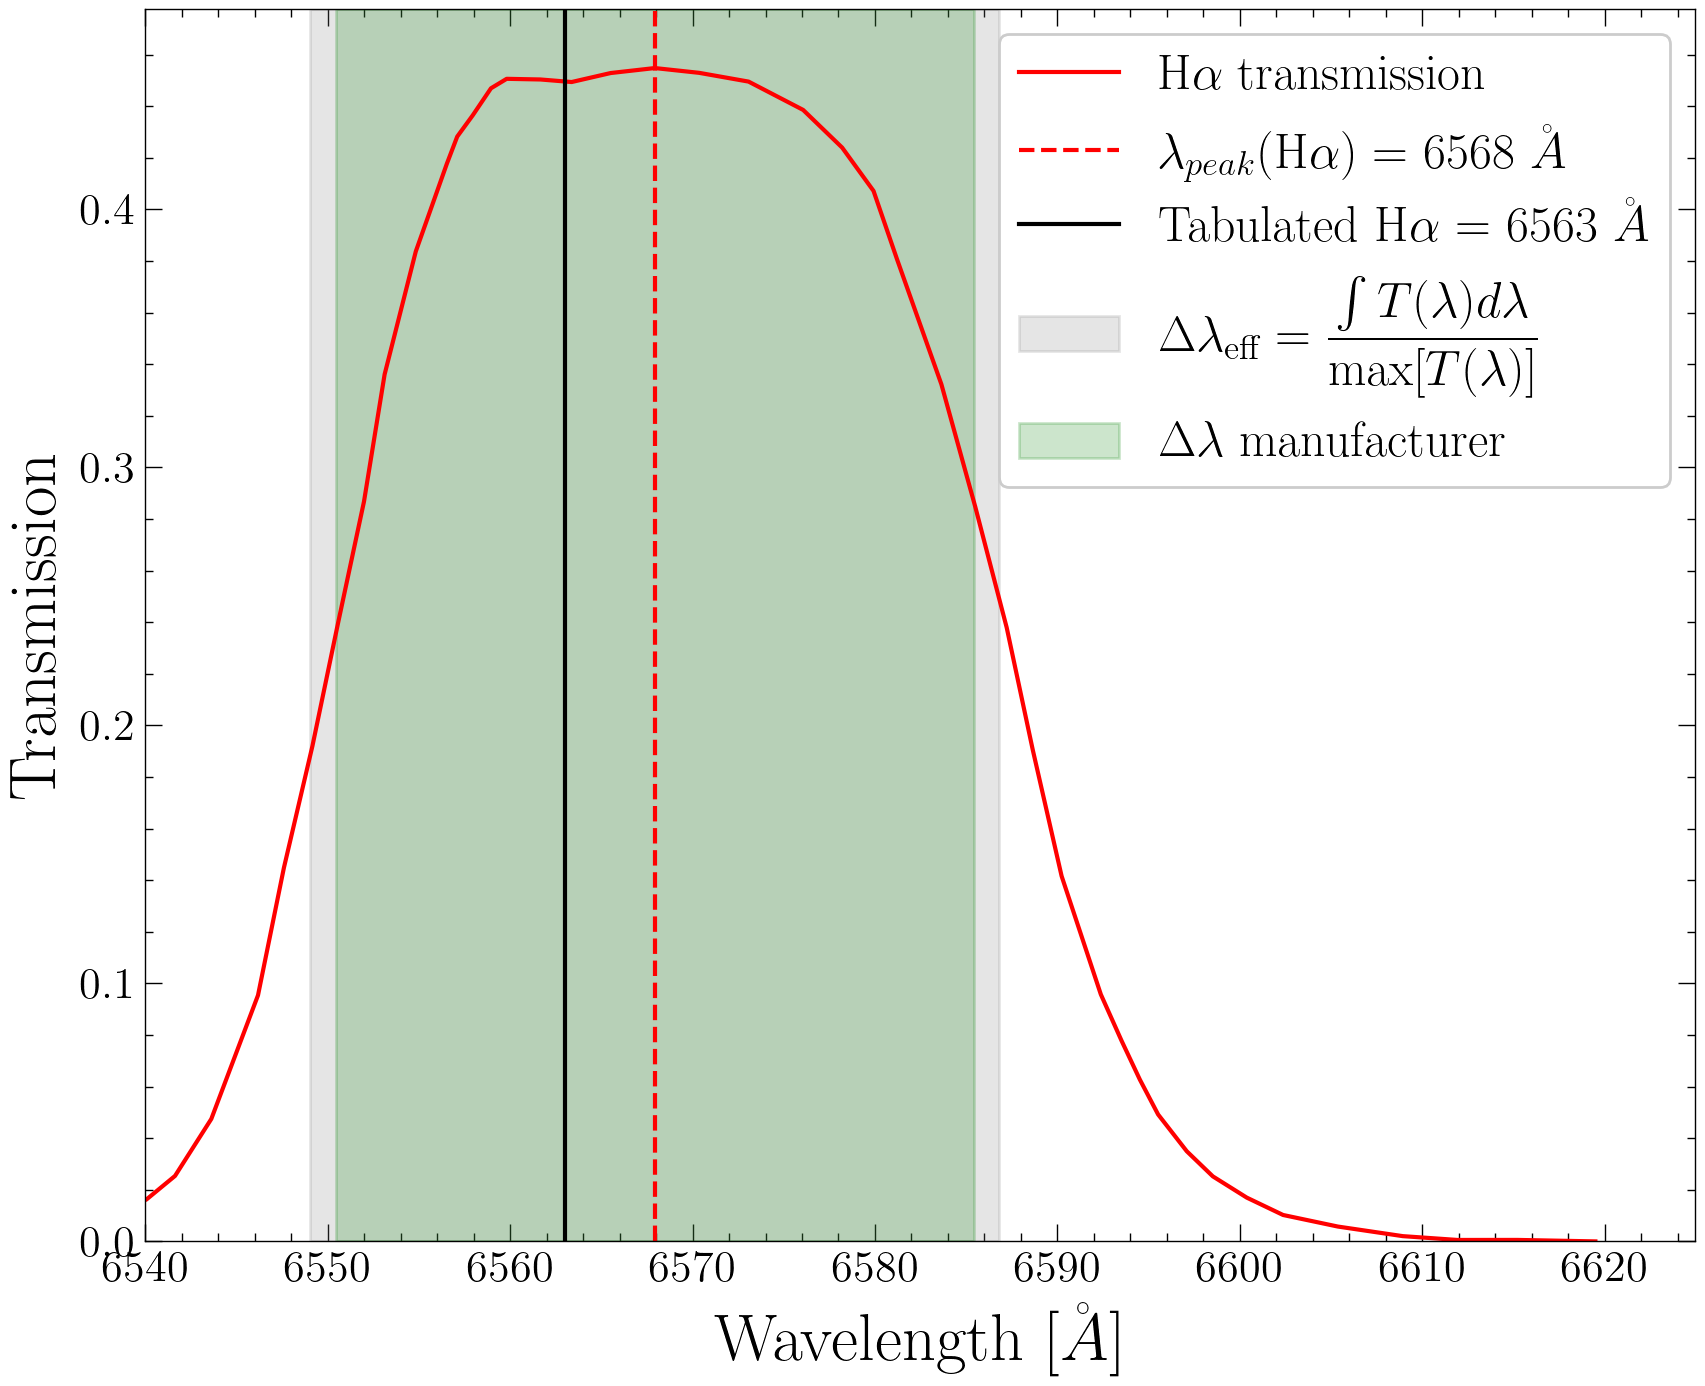
\includegraphics[width=0.95\columnwidth]{Ha_transmission.png}
    \caption{Transmission of the H$\alpha$ filter used in the observations.}
    \label{fig:Ha_transmission}
\end{figure}

\begin{figure}\centering
	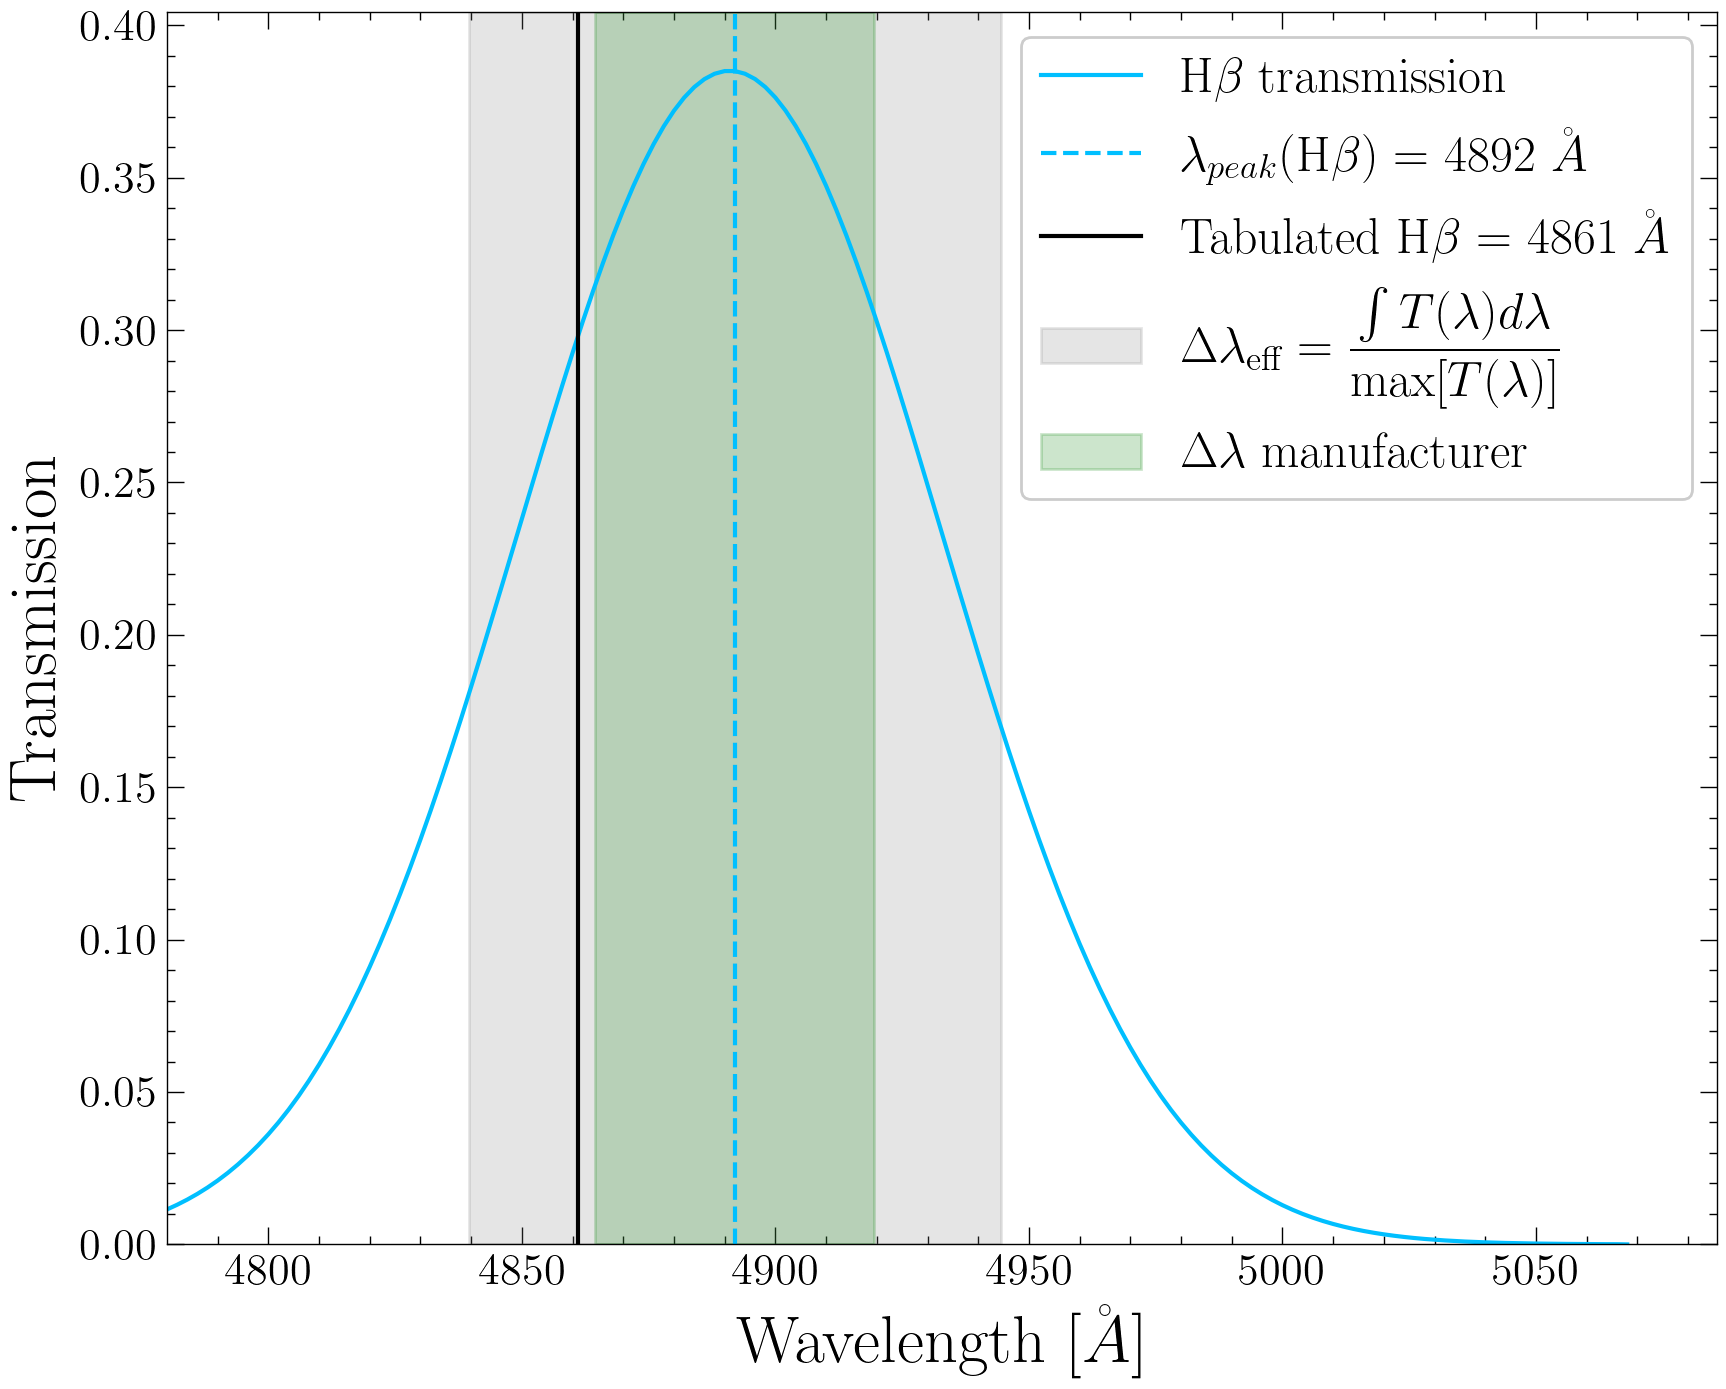
\includegraphics[width=0.95\columnwidth]{Hb_transmission.png}
    \caption{Transmission of the H$\beta$ filter used in the observations.}
    \label{fig:Hb_transmission}
\end{figure}

%%%%%%%%%%%%%%%%%%%%%%%%%%%%%%%%%%%%%%%%%%%%%%%%%%
%%%%%%%%%%%%%%%%%%%%%%%%%%%%%%%%%%%%%%%%%%%%%%%%%%%%%%%%%%%%%%%%%%%%%%%%%%%%%%%%%%%%%%%%%%%%%%%%%%%%


%%%%%%%%%%%%%%%%%%%% REFERENCES %%%%%%%%%%%%%%%%%%%%%%%%%%%%%%%%%%%%%%%%%%%%%%%%%%%%%%%%%%%%%%%%%%%%
% The best way to enter references is to use BibTeX:
\bibliographystyle{mnras}
\bibliography{bibliography} 
%%%%%%%%%%%%%%%%%%%%%%%%%%%%%%%%%%%%%%%%%%%%%%%%%%%%%%%%%%%%%%%%%%%%%%%%%%%%%%%%%%%%%%%%%%%%%%%%%%%%


% Don't change these lines
\label{lastpage}
\end{document}
